\chapter{Конструкторская часть}
В данном разделе будут приведены схемы алгоритмов нахождения расстояний Левенштейна и Дамерау-Левенштейна, приведено описание используемых типов данных, оценки памяти, а также описана структура ПО.

\section{Представление алгоритмов}

На вход алгоритмов падаются строки $S_{1}$ и $S_{2}$, на выходе ~---~ единственное число, искомое расстояние.

На рис. \ref{fig:L_rec} --- \ref{fig:DL_rec} приведены схемы рекурсивных и матричных алгоритмов нахождения расстояний Левенштейна и Дамерау-Левенштейна.

\clearpage

\begin{figure}[h]
	\centering
	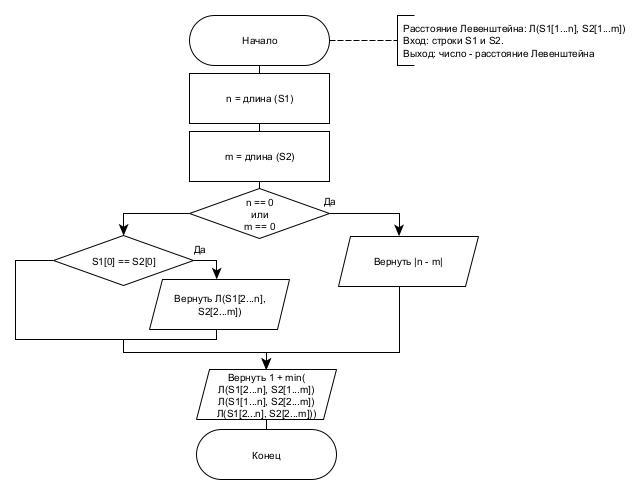
\includegraphics[scale=0.8]{img/levrec.jpg}
	\caption{Схема рекурсивного алгоритма нахождения расстояния Левенштейна}
	\label{fig:L_rec}
\end{figure}

\clearpage

\begin{figure}[h]
	\centering
	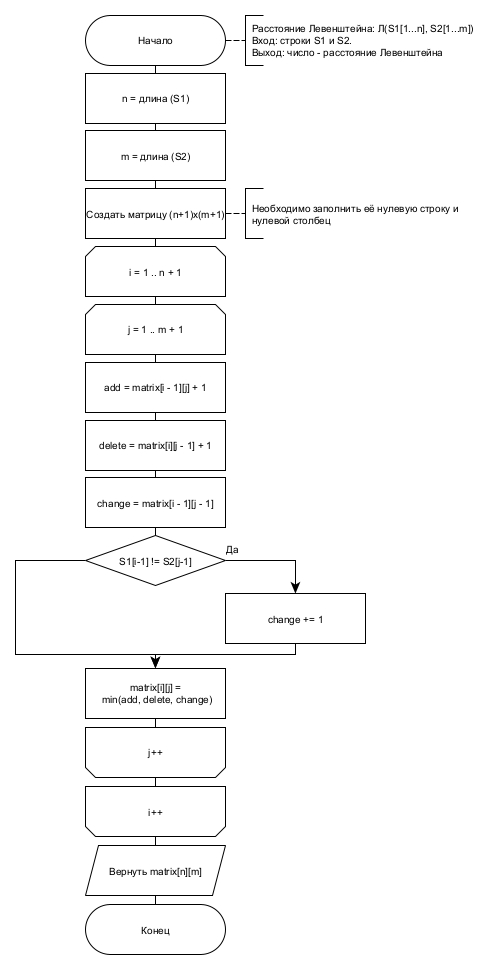
\includegraphics[scale=0.6]{img/levdyn.jpg}
	\caption{Схема динамического алгоритма нахождения расстояния Левенштейна}
	\label{fig:L_table}
\end{figure}

\clearpage

\begin{figure}[h]
	\centering
	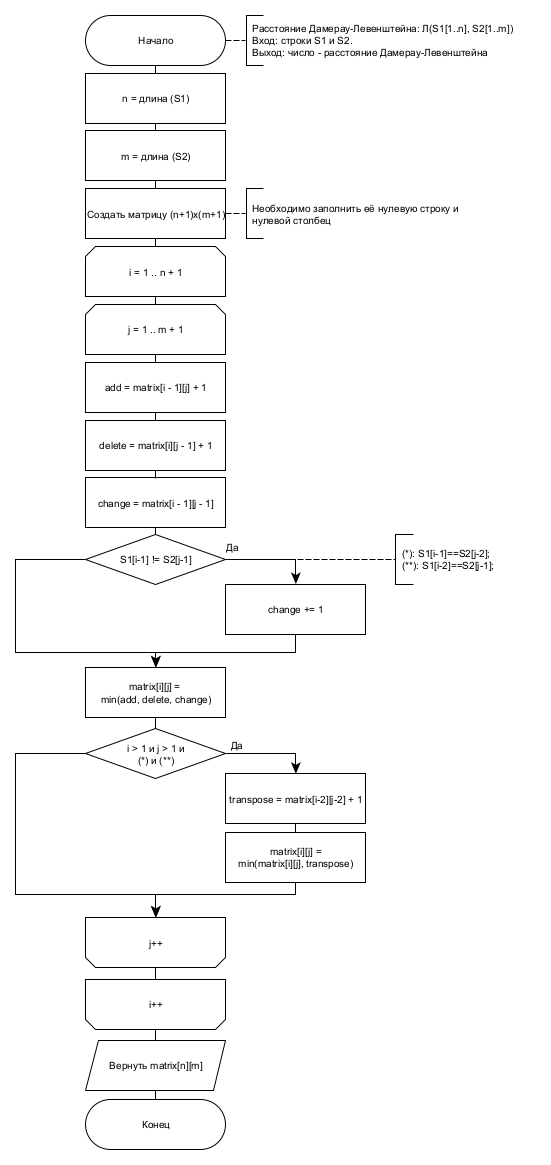
\includegraphics[scale=0.6]{img/damlevdyn.jpg}
	\caption{Схема динамического алгоритма нахождения расстояния Дамерау-Левенштейна}
	\label{fig:DL_rec}
\end{figure}

\clearpage

\textbf{ВЫВОД}

 В данном разделе были представлены схемы алгоритмов нахождения расстояний Левенштейна и Дамерау-Левенштейна.

\clearpage